% Ferdowsi: ML/DL for IoT-Enabled Smart Home Systems
%
% COMPILE:  lualatex main.tex  &&  lualatex main.tex
% (a second pass is required to resolve cross-references and citations;
%  lualatex is required for the banner/folio overlay and bundled fonts.
%  All fonts and images are bundled under assets/, so no system font
%  installation is needed.)
\documentclass[11pt,a4paper]{article}

\usepackage{fontspec}
\setmainfont{LiberationSerif}[
  Path = assets/fonts/, Extension = .ttf,
  UprightFont = *-Regular, BoldFont = *-Bold,
  ItalicFont = *-Italic, BoldItalicFont = *-BoldItalic,
]
\newfontfamily\sansfont{LiberationSans}[
  Path = assets/fonts/, Extension = .ttf,
  UprightFont = *-Regular, BoldFont = *-Bold,
]

\usepackage[a4paper,top=1.97in,bottom=0.98in,left=0.9in,right=0.9in]{geometry}
\usepackage{amsmath,amssymb}
\usepackage[round,authoryear]{natbib}
\usepackage{graphicx}
\usepackage{caption}
\usepackage{subcaption}
\usepackage{booktabs}
\usepackage{array}
\usepackage[table]{xcolor}
\usepackage[colorlinks=true,linkcolor=black,citecolor=black,urlcolor={blue!50!black}]{hyperref}
\usepackage{titlesec}
\usepackage{enumitem}
\usepackage{setspace}
\usepackage{tikz}
\usetikzlibrary{arrows.meta,positioning,fit,shapes.geometric}
\usepackage{eso-pic}
\usepackage{placeins}
\usepackage{algorithm}
\usepackage{algpseudocode}

% Page furniture: full-bleed conference banner + oversized folio, repeated
% on every page via eso-pic.
\definecolor{tablehead}{HTML}{8DB3E2}
\newlength{\bannerheight}
\setlength{\bannerheight}{0.2132813\paperwidth}
\AddToShipoutPictureBG{%
  \AtPageUpperLeft{\raisebox{-\bannerheight}[0pt][0pt]{
\includegraphics[width=\paperwidth]{assets/header_banner.jpeg}}}%
}
\AddToShipoutPictureFG{%
  \AtPageUpperLeft{\hspace*{0.3in}\raisebox{-385.7pt}[0pt][0pt]{\sffamily\fontsize{24}{24}\selectfont\textcolor{black!75}{\thepage}}}%
}

% The template's folio is the oversized digit in the left margin above;
% suppress LaTeX's own bottom-center page number so it isn't duplicated.
\pagestyle{empty}

\setlength{\parindent}{0pt}
\setlength{\parskip}{6pt}
\singlespacing
\raggedbottom

% Heading sizes per the template's type spec: section titles 12pt bold,
% subtitles 11pt bold.
\titleformat{\section}{\bfseries\fontsize{12}{14}\selectfont}{\thesection.}{0.5em}{}
\titleformat{\subsection}{\bfseries\fontsize{11}{13}\selectfont}{\thesubsection}{0.5em}{}
\titlespacing*{\section}{0pt}{1.3em}{0.55em}
\titlespacing*{\subsection}{0pt}{1.05em}{0.4em}

\captionsetup{font=footnotesize,labelfont={bf,footnotesize},skip=6pt}

\begin{document}

% ------------------------------------------------------------------ %
% Title / authors
% ------------------------------------------------------------------ %
\begin{center}
{\bfseries\fontsize{16}{19}\selectfont Machine Learning and Deep Learning for IoT-Enabled Smart Home Systems:\\[2pt]
An Integrated Architecture for Energy Forecasting, Occupancy Sensing, and Prescriptive Energy Management}

\vspace{1em}
{\bfseries\fontsize{12}{14}\selectfont Anita Ganji Moghadam$^{1,2}$}\\
\fontsize{11}{13}\selectfont
$^{1}$Department of Computer Engineering, Ferdowsi University of Mashhad --- anita.ganjimoghadam@mail.um.ac.ir\\
$^{2}$GreenWeb Corp --- a.ganjimoghadam@greenweb.ir

\vspace{0.6em}
{\bfseries\fontsize{12}{14}\selectfont Mohammadreza Sharifi$^{1,3}$}\\
\fontsize{11}{13}\selectfont
$^{1}$Department of Computer Engineering, Ferdowsi University of Mashhad --- sharifi.mohammadreza@mail.um.ac.ir\\
$^{3}$Iranserver Inc --- mr.sharifi@iranserver.com
\end{center}

\vspace{0.6em}
\noindent{\bfseries\fontsize{12}{14}\selectfont Abstract}

\begingroup
\fontsize{12}{15}\selectfont\itshape
\noindent The growth of Internet of Things (IoT) infrastructure in residential environments has produced continuous streams of energy, environmental, and occupancy data, creating an opportunity to apply machine learning (ML) to real household decision-making. This paper presents Ferdowsi, a full-stack smart-home platform that couples a React-based IoT dashboard -- covering device control, room-level monitoring, security, automation, and multi-utility energy visualization -- with a Django REST backend hosting three trained ML components: (i) a 48-hour household energy forecasting module combining a multi-output Random Forest regressor with Holt-Winters exponential smoothing and a disagreement-based 95\% prediction interval; (ii) a room-occupancy detection module trained on ambient sensor features (temperature, humidity, light, CO$_2$) using Random Forest and Logistic Regression classifiers; and (iii) a prescriptive energy-management agent trained with tabular Q-learning over a custom Markov Decision Process that recommends hourly load-shifting, battery-charging, and discharging actions. All three components are trained on public UCI datasets or a documented simulation environment, served through a versioned REST API, containerized with Docker and nginx, and consumed live by the dashboard. On held-out data, the Random Forest forecaster reduces mean absolute error by 9.5\% relative to a seasonal-naive baseline, the Logistic Regression occupancy classifier reaches 99.0\% accuracy and 0.995 ROC-AUC, and the learned Q-learning policy improves average episodic return by 1.23 units over a fixed-schedule heuristic and by 4.51 units over an always-idle baseline. Beyond these results, the paper documents the platform's feature inventory, deployment architecture, and internal, external, and construct validity limitations, and offers the system as a reproducible reference architecture for ML-driven IoT smart-home research.
\endgroup

\vspace{0.4em}
\noindent{\bfseries\fontsize{12}{14}\selectfont Keywords:} \fontsize{12}{14}\selectfont Internet of Things (IoT), Smart Home, Machine Learning, Deep Learning, Energy Forecasting, Occupancy Detection, Reinforcement Learning

% ------------------------------------------------------------------ %
\section{Introduction}

The Internet of Things has turned the residential environment into a continuously instrumented system, in which connected sensors and actuators generate high-frequency data on power consumption, occupancy, temperature, and appliance state. Converting this raw stream into actionable intelligence -- forecasting future demand, sensing where occupants are, and prescribing control actions -- is a central problem at the intersection of IoT and machine learning research. Most academic smart-home ML studies evaluate a single model in isolation on a benchmark dataset; fewer works integrate forecasting, perception, and decision-making into one deployed, end-to-end system that a real dashboard can consume in real time.

This paper presents such an integrated system: a full-stack smart-home dashboard, Ferdowsi, extended with three ML-backed capabilities -- (A) short-term household energy forecasting, (B) room-occupancy prediction, and (C) prescriptive energy management via reinforcement learning -- layered on an already feature-rich IoT dashboard covering device automation, multi-utility energy visualization, security, and geolocation-based presence. Each capability is trained on a public dataset or a documented simulation, served by a Django REST backend, and consumed by a React frontend, giving a reproducible reference architecture rather than an offline notebook study.

The remainder of the paper is organized as follows. Section 2 reviews related work. Section 3 describes the system architecture and feature inventory, including the deployment pipeline. Section 4 formalizes the three ML problems and the models used. Section 5 describes the datasets and experimental setup. Section 6 reports experimental results. Section 7 discusses limitations and threats to validity. Section 8 concludes and outlines future work.

\section{Related Work}

IoT-based smart-home intelligence draws on several largely separate research strands, reviewed below along the same three axes this paper contributes to, followed by a discussion of the IoT/smart-home systems literature and the gap this paper addresses.

\textbf{Residential and building energy forecasting.} Classical statistical forecasting of electricity demand has relied on autoregressive and exponential-smoothing families for decades: Box--Jenkins ARIMA modeling \citep{box1970} and the additive/multiplicative exponential smoothing methods of \citet{holt2004} and \citet{winters1960}, whose modern state of the art is surveyed by \citet{gardner2006}. These methods remain competitive baselines precisely because residential load at the single-household scale is noisy and behavior-driven rather than strongly seasonal, a point returned to in Section 6.1. Tree ensembles have been applied directly to short-term load forecasting with success -- e.g., \citet{lahouar2015} use a Random Forest with expert-guided feature selection for day-ahead load forecasting -- motivating the Random Forest component of this paper's ensemble. More recently, deep sequence models have become the default for load forecasting at scale: \citet{kong2019} show an LSTM recurrent network outperforming classical baselines on residential smart-meter data, but such gains are typically reported on multi-household or multi-year corpora; at the scale of one household's four-year history (the UCI dataset used here, \citealp{hebrail2012}), the bias--variance trade-off favors classical estimators, a design choice this paper makes explicit rather than treating as a limitation. Should a deep sequence model be trained as the corpus grows (Section 8), the cost of doing so need not scale with the full data volume: guided, informativeness-driven sample selection during training, such as the spectral data-selection method of \citet{sharifi2026}, has been shown to cut deep-network training cost substantially without sacrificing accuracy, and is a natural fit for keeping such an extension computationally tractable.

\textbf{Occupancy and presence sensing.} The UCI Occupancy Detection dataset introduced by \citet{candanedo2016} established Random Forest, gradient boosting, and linear discriminant models as strong baselines on ambient light/temperature/humidity/CO$_2$ features, a result this paper's own comparison (Section 6.2) is consistent with. \citet{ryu2016} broaden the comparison across support vector machines, Random Forests, and artificial neural networks for occupancy prediction from indoor environmental data in office buildings, likewise finding that simple, well-regularized classifiers are competitive once informative features (particularly light and CO$_2$) are available. Broader IoT smart-home surveys \citep{alaa2017} catalog occupancy and presence sensing as one of several core sensing modalities alongside energy, security, and health monitoring, but rarely connect it to a live control loop -- a gap this paper's Map-page occupancy panel and its documented single-room-to-multi-room extrapolation caveat (Section 4.2, Section 7) speak to directly.

\textbf{Reinforcement learning for demand response and building energy management.} The Markov Decision Process formalism \citep{bellman1957} and tabular Q-learning \citep{watkins1989,watkins1992} underlie nearly all RL-based home energy management work, with \citet{sutton2018} providing the standard modern treatment. Deep reinforcement learning, beginning with the Deep Q-Network of \citet{mnih2015}, extended these methods to large or continuous state spaces and has since been applied directly to building energy optimization: \citet{mocanu2019} train a deep RL agent for building-level load scheduling, and \citet{vazquezcanteli2019} survey a wide range of RL algorithms and state/action/reward formulations for demand response, noting that most reported gains come from settings with state spaces too large to enumerate. The energy-management agent in this paper occupies the opposite end of that spectrum -- a state space small enough to represent and update exactly in a table (Section 4.3) -- so the deep RL literature is used here to justify \emph{not} reaching for a neural policy, rather than as a method this paper extends.

\textbf{Integrated IoT smart-home systems.} Survey work on smart-home architectures \citep{alaa2017} documents a broad and mature ecosystem of dashboards, automation rules, and device-control layers, but the ML/DL components in that literature are typically evaluated offline, one at a time, disconnected from a deployed control surface. The contribution of this paper is not a new algorithm in any of the three strands above, but a single deployed, cross-strand architecture in which forecasting, perception, and control share one dashboard, one backend, and one persistence layer, with all three trained models served through a common REST API design and every choice of classical model over a deep one justified against the literature reviewed here rather than left implicit.

\section{System Architecture and Feature Inventory}

The platform follows a three-tier architecture, shown in Figure~\ref{fig:architecture}. A React 19 single-page application (the dashboard) communicates over a versioned REST API with a Django 4.2 / Django REST Framework backend, which hosts three independent Django apps -- \texttt{forecasting}, \texttt{occupancy}, and \texttt{energy\_manager} -- each wrapping a trained scikit-learn/statsmodels model or a hand-rolled Q-learning agent behind an inference endpoint. Trained model artifacts and the SQLite persistence layer are containerized with Docker for reproducible deployment.

\begin{figure}[htbp]
\centering
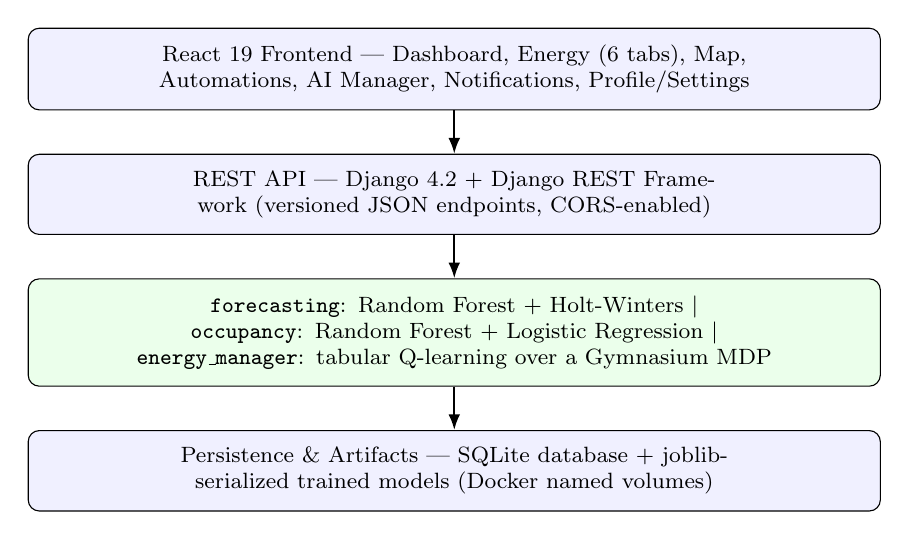
\begin{tikzpicture}[
  node distance=0.55cm,
  box/.style={draw, rounded corners, fill=blue!6, align=center, text width=10.4cm, minimum height=0.95cm, font=\footnotesize, inner sep=6pt},
  arr/.style={-{Latex[length=2mm]}, thick}
]
\node[box] (frontend) {React 19 Frontend --- Dashboard, Energy (6 tabs), Map, Automations, AI Manager, Notifications, Profile/Settings};
\node[box, below=of frontend] (api) {REST API --- Django 4.2 + Django REST Framework (versioned JSON endpoints, CORS-enabled)};
\node[box, below=of api, fill=green!8] (ml) {\texttt{forecasting}: Random Forest + Holt-Winters $\mid$ \texttt{occupancy}: Random Forest + Logistic Regression $\mid$ \texttt{energy\_manager}: tabular Q-learning over a Gymnasium MDP};
\node[box, below=of ml] (store) {Persistence \& Artifacts --- SQLite database + joblib-serialized trained models (Docker named volumes)};
\draw[arr] (frontend) -- (api);
\draw[arr] (api) -- (ml);
\draw[arr] (ml) -- (store);
\end{tikzpicture}
\caption{Three-tier system architecture: React frontend, Django REST backend, and the three ML/RL model apps, backed by SQLite and Docker-managed model artifacts.}
\label{fig:architecture}
\end{figure}

\subsection{Dashboard (root route)}

The main dashboard exposes a device grid with per-device on/off toggles persisted to local storage; room cards summarizing per-room devices, temperature, and humidity; a security-status card and a presence card showing which family members are home; a network-status card; an energy-distribution overview widget; an interactive floor plan with clickable room markers; a draggable dual-setpoint thermostat control; a rule-based AI insights panel that reasons over live application state; a scripted AI security assistant that detects a simulated break-in condition (motion while away) and autonomously locks doors and arms security, with state changes driven by a scripted, not inferred, reasoning trace; a combined activity log merging seeded history with a live notification stream; and modal dialogs for device management and change-history auditing.

\subsection{Energy Page (six tabs)}

The Energy page organizes utility data into six tabs: (1) \emph{Summary} -- daily solar/grid/battery/cost stat cards, an energy-distribution diagram, a sources table, a power-sources line chart, a stacked electricity-usage bar chart, and gas/water charts; (2) \emph{Electricity} -- a full usage breakdown, a solar-production chart, per-device usage charts, a hover-to-highlight Sankey-style power-flow diagram, a grid-balance bar, gauge donuts for net-imported energy, self-consumed solar percentage, and self-sufficiency percentage, and a detailed sources table; (3) \emph{Gas} -- consumption chart, period bar, and totals; (4) \emph{Water} -- consumption chart, period bar, and totals; (5) \emph{Now} -- a simulated live power feed (a bounded random walk updated every two seconds) driving live solar/grid/battery stat cards, a full-day power chart built up to the current time, live gauges, and a live power-flow diagram; and (6) \emph{Forecast} -- the ML-backed 48-hour ensemble energy forecast described in Section 4.1, rendered with a 95\% prediction-interval band, an hour-by-hour data table, a what-if scenario tool for simulating an appliance run at a chosen hour, and model test-metric chips.

\subsection{Map, Automations, AI Manager, and Supporting Pages}

The Map page renders a Leaflet map with a home-zone radius circle and family-member presence markers, overlaid with the ML-backed Predicted Occupancy panel described in Section 4.2, refreshed every 30 seconds. The Automations page lists trigger-condition-action rules and scene-activation cards. The AI Manager page (Section 4.3) exposes hour and battery-charge input controls, the current recommended action with a plain-language explanation and state chip, accept/reject controls that persist the operator's decision, a bar chart of the learned Q-value for every candidate action in the current state, and a full recommendation-history table. A persistent notification center records every meaningful state change across the application. The Profile and Settings pages provide theme, timezone, locale, and date/time-format preferences.

\subsection{Deployment Architecture}

The full stack is containerized with Docker: a multi-stage frontend image compiles the Vite/React application and serves the static bundle with nginx, which also reverse-proxies \texttt{/api} and \texttt{/admin} requests to the backend container; a backend image runs Django migrations, trains any missing ML artifact on first boot, and serves the API with gunicorn. A \texttt{docker-compose.yml} file orchestrates both services with named volumes for the SQLite database and trained model artifacts, and a one-command \texttt{run.sh} wrapper (\texttt{up}/\texttt{stop}/\texttt{down}/\texttt{reset}/\texttt{logs}) is provided for reproducible local or server deployment.

\begin{table}[htbp]
\centering
\caption{Technology stack}
\label{tab:stack}
\footnotesize
\renewcommand{\arraystretch}{1.3}
\begin{tabular}{@{}p{2.6cm}p{10cm}@{}}
\toprule
\rowcolor{tablehead}
\textbf{Layer} & \textbf{Technologies} \\
\midrule
Frontend & React 19, React Router 7, Vite, Chart.js/react-chartjs-2, Leaflet/react-leaflet \\
Backend & Django 4.2, Django REST Framework, django-cors-headers, SQLite \\
Machine Learning & scikit-learn, statsmodels, pandas, numpy, joblib \\
Reinforcement Learning & Gymnasium (custom environment), hand-rolled tabular Q-learning \\
Deployment & Docker, docker-compose, nginx, gunicorn \\
\bottomrule
\end{tabular}
\renewcommand{\arraystretch}{1}
\end{table}

\FloatBarrier
\section{Machine Learning and Deep Learning Methodology}

\subsection{Direction A --- Household Energy Forecasting}

Given an hourly household active-power series $y_t$, the forecasting module predicts the next $H=48$ hours directly (multi-horizon regression, not recursive one-step-ahead rollout) from a 72-hour lookback window and an engineered feature vector combining three sub-metering channels and cyclically encoded calendar features:

\begin{equation}
x_t = \left[\, y_t,\ s_t^1,\ s_t^2,\ s_t^3,\ \sin\!\left(\tfrac{2\pi h_t}{24}\right),\ \cos\!\left(\tfrac{2\pi h_t}{24}\right),\ \sin\!\left(\tfrac{2\pi d_t}{7}\right),\ \cos\!\left(\tfrac{2\pi d_t}{7}\right) \right]
\label{eq:forecast_features}
\end{equation}

Two structurally different models are trained and combined by simple averaging. The first is a multi-output Random Forest regressor \citep{breiman2001,breiman1984} with $B=80$ trees and maximum depth 10, whose prediction $\hat f(x)$ is the mean over trees, each grown by the standard multi-output extension of the CART variance-reduction splitting rule \citep{breiman1984}. The second is a Holt-Winters exponential smoothing model \citep{winters1960,holt2004} with no trend term and a multiplicative seasonal component of period $m=24$ -- chosen, unlike an additive or trended variant, because it structurally cannot produce negative forecasts on this non-negative series. Its level $\ell_t$ and seasonal index $s_t$ are updated recursively and combined into the $h$-step-ahead forecast as

\begin{equation}
\hat y_{t+h} = \ell_t \cdot s_{t+h-m\lceil h/m \rceil}.
\label{eq:hw}
\end{equation}

A 95\% prediction interval is derived from the disagreement between the two ensemble members rather than either model's own parametric uncertainty, a pragmatic substitute for quantile regression or Monte Carlo dropout for a two-member classical-ML ensemble:

\begin{equation}
\sigma_{t+h} = \frac{\left| \hat y_{t+h}^{\mathrm{RF}} - \hat y_{t+h}^{\mathrm{HW}} \right|}{\sqrt{2}}, \qquad
\mathrm{PI}_{95\%} = \hat y_{t+h}^{\mathrm{ens}} \pm 1.96\,\sigma_{t+h}
\label{eq:pi}
\end{equation}

Forecast accuracy is measured on the held-out test set, across all $N$ windows and $H=48$ horizon steps, by the standard mean absolute error and root-mean-squared error, against a seasonal-naive baseline ($\hat y_{t+h} = y_{t+h-24}$, i.e. repeating the same hour one day earlier), used as the minimum bar for usefulness following standard practice in the M4/M5 forecasting-competition literature \citep{makridakis2020}. Both models are fit with off-the-shelf, widely validated implementations -- scikit-learn's \texttt{RandomForestRegressor} \citep{pedregosa2011} and statsmodels' \texttt{ExponentialSmoothing} \citep{seabold2010} -- rather than hand-rolled estimators, so the fit times reported in Table~\ref{tab:forecast_results} reflect production-grade code, not a research prototype.

\subsection{Direction B --- Room Occupancy Detection}

Occupancy is formulated as binary classification over a seven-dimensional feature vector of ambient sensor readings and calendar features:

\begin{equation}
x_t = \left[\, \mathrm{Temperature}_t,\ \mathrm{Humidity}_t,\ \mathrm{Light}_t,\ \mathrm{CO2}_t,\ \mathrm{HumidityRatio}_t,\ h_t,\ d_t \,\right]
\label{eq:occ_features}
\end{equation}

A Random Forest classifier (200 trees, depth 10, class-balanced to correct for the $\sim$23\% occupied-class prevalence) minimizes Gini impurity at each split \citep{breiman1984}. A Logistic Regression classifier \citep{cox1958,hosmer2013} is trained as a second, structurally different ensemble member, whose disagreement with the Random Forest flags borderline cases: it models the occupancy probability as a sigmoid of a linear score in the seven features of Eq.~\eqref{eq:occ_features}, with weights fit by $\ell_2$-regularized, class-balanced maximum-likelihood estimation (L-BFGS, \texttt{max\_iter}=1000).

Both classifiers are evaluated with the standard binary-classification suite -- accuracy, precision, recall, F1, and threshold-independent ROC-AUC, the last summarizing the true-/false-positive-rate trade-off across every classification threshold. Random Forest feature importances are likewise the standard mean Gini-impurity decrease attributable to each feature across the forest \citep{breiman1984}.

Per-room estimates on the dashboard's six simulated rooms are produced by evaluating the single-room-trained classifier on schema-matched feature vectors synthesized from each room's known temperature, humidity, and light state. This is a sensitivity analysis of the trained model, not validated per-room ground truth, and is stated explicitly as such in Section 7.

\subsection{Direction C --- Prescriptive Energy Management via Reinforcement Learning}

The energy-management agent operates over a finite-horizon Markov Decision Process $(S, A, P, R, \gamma)$ \citep{bellman1957} representing one simulated household day. The state $s=(h,p,u,b) \in \{0,\dots,23\} \times \{0,1,2\}^3$ is a four-tuple of discretized hour, grid-price tier, solar-output tier, and battery state-of-charge tier, giving $|S|=24\times3\times3\times3=648$; the action space $A=\{\texttt{idle}, \texttt{run\_load}, \texttt{charge}, \texttt{discharge}\}$ has $|A|=4$ members, so the full state-action space has $|S|\times|A|=2{,}592$ entries -- small enough to enumerate exactly, unlike the state spaces deep RL is typically justified by \citep{mnih2015,vazquezcanteli2019}. The environment is implemented as a custom Gymnasium \citep{towers2024} environment, following the interface introduced by OpenAI Gym \citep{brockman2016}. The reward at each hour combines a time-of-use grid-cost term with a one-time completion bonus for the flexible load and a terminal discomfort penalty if it never runs:

\begin{equation}
r_t =
\begin{cases}
-\,p(h_t)\,g_t \;+\; \beta, & a_t = \texttt{run\_load} \text{ and the load has not yet run}, \\[2pt]
-\,p(h_t)\,g_t, & \text{otherwise},
\end{cases}
\label{eq:reward}
\end{equation}

with a one-time terminal penalty $r_T \mathrel{-}= \kappa$ if the flexible load never ran, where $p(h_t)$ is the time-of-use grid price, $g_t$ the grid energy drawn that hour, $\beta=0.5$ the on-time bonus, $\kappa=3.0$ the terminal penalty, and $T=24$ the episode length. A tabular Q-learning agent \citep{watkins1989,watkins1992} is trained with the standard temporal-difference update rule

\begin{equation}
Q(s_t,a_t) \leftarrow Q(s_t,a_t) + \alpha\left[ r_t + \gamma \max_{a'} Q(s_{t+1},a') - Q(s_t,a_t) \right],
\label{eq:qlearning}
\end{equation}

with learning rate $\alpha=0.1$, discount $\gamma=0.95$, and an $\varepsilon$-greedy behavior policy (Algorithm~\ref{alg:qlearning}) decaying linearly from 1.0 to 0.05 over the first 3,000 of 4,000 training episodes; under the standard convergence conditions for this update \citep{watkins1992}, it is guaranteed to reach the optimal action-value function since $S$ and $A$ are finite and every state-action pair is visited infinitely often. Given the small, fully enumerable $|S|\times|A|=2{,}592$-entry state-action space, a tabular representation is the exact optimal representation for this MDP; a deep Q-network \citep{mnih2015} offers no representational benefit at this scale, so the classical formulation is used by design rather than by omission.

\begin{algorithm}[htbp]
\caption{Tabular Q-learning for the home energy management MDP}
\label{alg:qlearning}
\begin{algorithmic}[1]
\State Initialize $Q(s,a) \gets 0$ for all $s \in S,\, a \in A$
\For{episode $= 1, \dots, N_{\text{episodes}}$}
  \State $\varepsilon \gets \varepsilon_{\text{start}} + \min(1, \text{episode}/N_{\text{decay}}) \cdot (\varepsilon_{\text{end}} - \varepsilon_{\text{start}})$
  \State Reset environment; observe initial state $s_0$
  \For{$t = 0, 1, \dots$ until episode terminates}
    \State $a_t \gets$ a uniformly random action with probability $\varepsilon$, else $\arg\max_{a} Q(s_t, a)$
    \State Execute $a_t$; observe reward $r_t$ (Eq.~\eqref{eq:reward}) and next state $s_{t+1}$
    \State $Q(s_t,a_t) \gets Q(s_t,a_t) + \alpha\left[r_t + \gamma \max_{a'} Q(s_{t+1},a') - Q(s_t,a_t)\right]$
  \EndFor
\EndFor
\State \Return greedy policy $\pi(s) = \arg\max_{a} Q(s,a)$
\end{algorithmic}
\end{algorithm}

\FloatBarrier
\section{Datasets and Experimental Setup}

\begin{table}[htbp]
\centering
\caption{Datasets used}
\label{tab:datasets}
\footnotesize
\renewcommand{\arraystretch}{1.3}
\begin{tabular}{@{}p{4.3cm}p{2.3cm}p{3.6cm}p{2.4cm}@{}}
\toprule
\rowcolor{tablehead}
\textbf{Dataset} & \textbf{Used by} & \textbf{Size} & \textbf{Source} \\
\midrule
UCI Individual Household Electric Power Consumption & Forecasting & 2{,}075{,}259 minute-level rows ($\sim$34k hourly after resampling) & \citet{hebrail2012} \\
UCI Occupancy Detection Dataset & Occupancy & 8{,}143 train + 12{,}417 test rows & \citet{candanedo2016} \\
Custom Gymnasium MDP simulation & Energy management & n/a (simulated) & hand-crafted price/solar/battery model \\
\bottomrule
\end{tabular}
\renewcommand{\arraystretch}{1}
\end{table}

Forecasting and occupancy models are evaluated on genuine held-out splits: a chronological 80/10/10 train/validation/test split ($n_{\mathrm{train}}=30{,}671$ windows, $n_{\mathrm{test}}=3{,}302$ windows, no shuffling) for forecasting, and the occupancy dataset's own published train/test split for occupancy. The energy-management agent is evaluated on 200 freshly sampled episodes from the same simulated environment distribution used in training, since the environment itself is the ground truth rather than an approximation of external data. All experiments use fixed random seeds (\texttt{random\_state=42} / \texttt{seed=42}) for reproducibility; data loading and feature engineering use pandas \citep{mckinney2010}, models are fit with scikit-learn \citep{pedregosa2011} and statsmodels \citep{seabold2010}, and the code, trained artifacts, and figures in this paper were regenerated end-to-end from the repository at submission time.

\FloatBarrier
\section{Results and Discussion}

\subsection{Energy Forecasting}

\begin{table}[htbp]
\centering
\caption{Energy forecasting results (held-out test set, hourly kW, 48h-horizon windows)}
\label{tab:forecast_results}
\footnotesize
\begin{tabular}{@{}lccc@{}}
\toprule
\rowcolor{tablehead}
\textbf{Model} & \textbf{Test MAE (kW)} & \textbf{Test RMSE (kW)} & \textbf{Fit time} \\
\midrule
Random Forest (multi-output) & 0.457 & 0.603 & 4.1\,s \\
Holt-Winters (no trend, multiplicative) & 0.581 & 0.761 & 0.7\,s \\
Seasonal-naive baseline & 0.505 & 0.764 & --- \\
\bottomrule
\end{tabular}
\end{table}

\begin{figure}[htbp]
\centering
\begin{subfigure}[b]{0.58\textwidth}
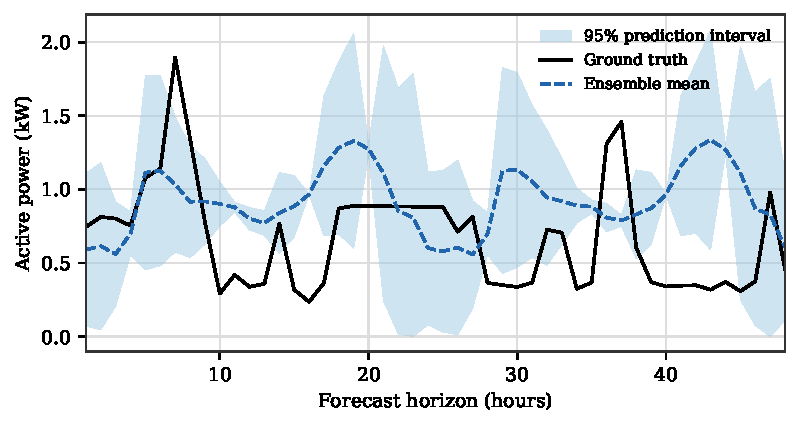
\includegraphics[width=\textwidth]{figures/forecast_pi.pdf}
\caption{}
\label{fig:forecast_pi}
\end{subfigure}
\hfill
\begin{subfigure}[b]{0.38\textwidth}
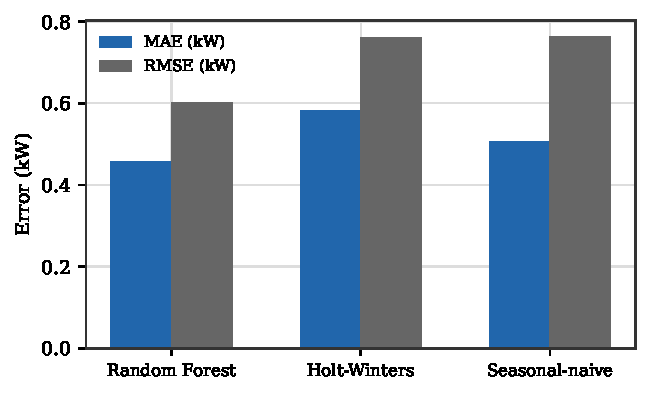
\includegraphics[width=\textwidth]{figures/forecast_error_bars.pdf}
\caption{}
\label{fig:forecast_bars}
\end{subfigure}
\caption{(a) A representative 48-hour ensemble forecast on the held-out test set, showing the ensemble mean, ground truth, and the disagreement-based 95\% prediction interval. (b) Test MAE and RMSE for the Random Forest, Holt-Winters, and seasonal-naive models.}
\label{fig:forecast}
\end{figure}

The Random Forest forecaster outperforms the seasonal-naive baseline on both metrics, a 9.5\% relative reduction in MAE. Holt-Winters is roughly tied with the naive baseline and is, in fact, slightly worse on MAE: a single-household power series is dominated by occupant behavior, which a smooth seasonal model does not capture, whereas Random Forest benefits from sub-metering and calendar context. The two-model ensemble's practical contribution is therefore the disagreement-based prediction interval shown in Figure~\ref{fig:forecast_pi} rather than an improvement in point-forecast accuracy; Random Forest should be read as the strongest standalone point forecaster in this comparison.

\subsection{Occupancy Detection}

\begin{table}[htbp]
\centering
\caption{Occupancy detection results (held-out test set, $n=12{,}417$)}
\label{tab:occupancy_results}
\footnotesize
\begin{tabular}{@{}lccccc@{}}
\toprule
\rowcolor{tablehead}
\textbf{Model} & \textbf{Accuracy} & \textbf{Precision} & \textbf{Recall} & \textbf{F1} & \textbf{ROC-AUC} \\
\midrule
Random Forest & 0.966 & 0.923 & 0.939 & 0.931 & 0.994 \\
Logistic Regression & 0.990 & 0.966 & 0.996 & 0.980 & 0.995 \\
\bottomrule
\end{tabular}
\end{table}

Logistic Regression outperforms Random Forest on every metric, which runs counter to the common expectation that tree ensembles dominate linear models on tabular data. Random Forest feature importances show Light (0.470) and CO$_2$ (0.212) jointly carrying 68\% of total importance, indicating that the occupancy-to-sensor relationship is close to linearly separable -- a regime in which a linear decision boundary is sufficient and a tree ensemble's additional capacity adds variance without adding accuracy. Both models' ROC-AUC of approximately 0.99 indicates that most of the achievable performance comes from the informativeness of the five-feature representation itself rather than from classifier choice, consistent with the original dataset paper \citep{candanedo2016}.

\subsection{Prescriptive Energy Management}

\begin{table}[htbp]
\centering
\caption{Prescriptive energy management results (200 held-out episodes, mean episodic return)}
\label{tab:energy_results}
\footnotesize
\begin{tabular}{@{}lccc@{}}
\toprule
\rowcolor{tablehead}
\textbf{Policy} & \textbf{Avg. return} & \textbf{vs. always-idle} & \textbf{vs. naive-fixed-time} \\
\midrule
Learned (Q-learning, greedy) & $+0.109$ & $+4.51$ & $+1.23$ \\
Naive fixed-time (load @ 8am) & $-1.123$ & $+3.28$ & --- \\
Always-idle & $-4.404$ & --- & --- \\
\bottomrule
\end{tabular}
\end{table}

\begin{figure}[htbp]
\centering
\begin{subfigure}[b]{0.46\textwidth}
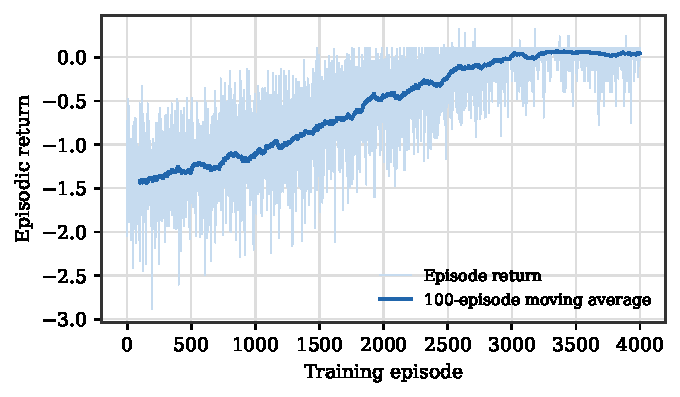
\includegraphics[width=\textwidth]{figures/energy_training_curve.pdf}
\caption{}
\label{fig:energy_curve}
\end{subfigure}
\hfill
\begin{subfigure}[b]{0.24\textwidth}
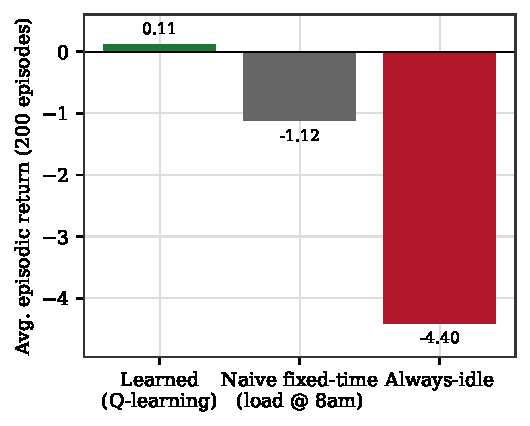
\includegraphics[width=\textwidth]{figures/energy_policy_comparison.pdf}
\caption{}
\label{fig:energy_policy}
\end{subfigure}
\hfill
\begin{subfigure}[b]{0.24\textwidth}
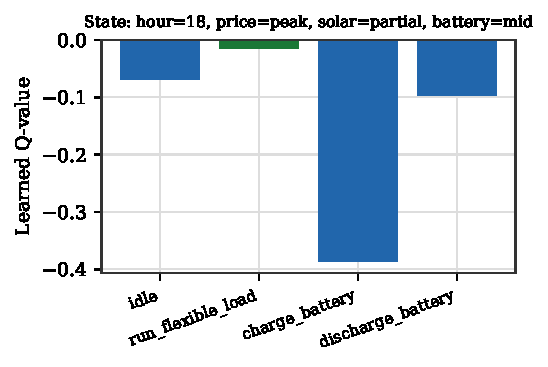
\includegraphics[width=\textwidth]{figures/energy_qvalues.pdf}
\caption{}
\label{fig:energy_qvalues}
\end{subfigure}
\caption{(a) Per-episode return during training and its 100-episode moving average, over 4,000 training episodes. (b) Average episodic return of the learned policy against both baselines over 200 held-out episodes. (c) Learned Q-values for each candidate action in a representative evening-peak state.}
\label{fig:energy}
\end{figure}

The learned policy outperforms both baselines. The gap against always-idle ($+4.51$) is dominated by the environment's discomfort penalty for never running the flexible load, so it is best read as evidence that the agent learns it must act, rather than as the paper's central result. The more informative comparison is against naive-fixed-time ($+1.23$), which isolates the value of conditioning the policy on price, solar, and battery state over a fixed-schedule heuristic a household could already follow without any learning.

\FloatBarrier
\section{Limitations and Threats to Validity}

Internal validity is supported by genuine held-out evaluation for both forecasting and occupancy, with no train/test leakage; the energy manager's held-out episodes are freshly sampled from the same training distribution, since the environment is itself the ground truth rather than external data, and this distinction is stated explicitly rather than left implicit. External validity is limited: the forecasting and occupancy models are trained on one household and one room respectively, so the reported metrics describe performance on that specific unit rather than households or rooms in general, and the energy manager's price, solar, and battery constants are hand-set rather than fit to a real household. Construct validity is most relevant to the multi-room occupancy extrapolation: per-room dashboard estimates come from evaluating a single-room-trained classifier on synthesized feature vectors and should be read as a sensitivity analysis of the model, not as validated multi-room ground truth. Finally, all reported numbers are single-seed point estimates; reporting mean $\pm$ standard deviation over multiple random seeds is the natural next step before treating these results as more than illustrative.

\section{Conclusion and Future Work}

This paper presented an integrated IoT-based smart-home platform that combines a full-featured dashboard -- device control, multi-utility energy visualization, security, automation, and geolocation-based presence -- with three trained machine-learning components covering energy forecasting, occupancy detection, and prescriptive reinforcement-learning-based energy management, deployed end-to-end and containerized for reproducible use. Each component is trained on a public dataset or a documented simulation and evaluated against an appropriate baseline. Results show consistent improvements over naive baselines across all three directions, alongside nuanced findings -- such as Holt-Winters underperforming a naive baseline on MAE, and a linear model outperforming a tree ensemble on occupancy -- that are informative in their own right for IoT machine-learning practitioners. Future work includes multi-seed statistical validation with confidence intervals, replacing the hand-set energy-management constants with values fit to real household telemetry, extending the occupancy model to a genuinely multi-room labeled dataset, and evaluating deep sequence models (LSTM/Temporal Convolutional Networks) against the current classical-ML forecasting ensemble as the training corpus grows beyond a single household -- at which point guided data-selection methods \citep{sharifi2026} become directly relevant to keeping that training affordable.

\begingroup
\small
\begin{thebibliography}{99}
\setlength{\itemsep}{0.3em}

\bibitem[Alaa et al.(2017)]{alaa2017} Alaa, M., Zaidan, A. A., Zaidan, B. B., Talal, M., \& Kiah, M. L. M. (2017). A review of smart home applications based on Internet of Things. \emph{Journal of Network and Computer Applications}, 97, 48--65.

\bibitem[Bellman(1957)]{bellman1957} Bellman, R. (1957). A Markovian Decision Process. \emph{Journal of Mathematics and Mechanics}, 6(5), 679--684.

\bibitem[Box \& Jenkins(1970)]{box1970} Box, G. E. P., \& Jenkins, G. M. (1970). \emph{Time Series Analysis: Forecasting and Control}. Holden-Day.

\bibitem[Breiman(2001)]{breiman2001} Breiman, L. (2001). Random Forests. \emph{Machine Learning}, 45(1), 5--32.

\bibitem[Breiman et al.(1984)]{breiman1984} Breiman, L., Friedman, J. H., Olshen, R. A., \& Stone, C. J. (1984). \emph{Classification and Regression Trees}. Wadsworth.

\bibitem[Brockman et al.(2016)]{brockman2016} Brockman, G., Cheung, V., Pettersson, L., Schneider, J., Schulman, J., Tang, J., \& Zaremba, W. (2016). OpenAI Gym. \emph{arXiv preprint} arXiv:1606.01540.

\bibitem[Candanedo \& Feldheim(2016)]{candanedo2016} Candanedo, L. M., \& Feldheim, V. (2016). Accurate occupancy detection of an office room from light, temperature, humidity and CO2 measurements using statistical learning models. \emph{Energy and Buildings}, 112, 28--39.

\bibitem[Cox(1958)]{cox1958} Cox, D. R. (1958). The regression analysis of binary sequences. \emph{Journal of the Royal Statistical Society, Series B}, 20(2), 215--242.

\bibitem[Gardner(2006)]{gardner2006} Gardner, E. S. (2006). Exponential smoothing: The state of the art---Part II. \emph{International Journal of Forecasting}, 22(4), 637--666.

\bibitem[Hebrail \& Berard(2012)]{hebrail2012} Hebrail, G., \& Berard, A. (2012). Individual Household Electric Power Consumption Data Set. \emph{UCI Machine Learning Repository}. \url{https://archive.ics.uci.edu/dataset/235}

\bibitem[Holt(2004)]{holt2004} Holt, C. C. (2004). Forecasting seasonals and trends by exponentially weighted moving averages. \emph{International Journal of Forecasting}, 20(1), 5--10. (Reprint of 1957 ONR Research Memorandum 52.)

\bibitem[Hosmer et al.(2013)]{hosmer2013} Hosmer, D. W., Lemeshow, S., \& Sturdivant, R. X. (2013). \emph{Applied Logistic Regression} (3rd ed.). Wiley.

\bibitem[Kong et al.(2019)]{kong2019} Kong, W., Dong, Z. Y., Jia, Y., Hill, D. J., Xu, Y., \& Zhang, Y. (2019). Short-term residential load forecasting based on LSTM recurrent neural network. \emph{IEEE Transactions on Smart Grid}, 10(1), 841--851.

\bibitem[Lahouar \& Ben Hadj Slama(2015)]{lahouar2015} Lahouar, A., \& Ben Hadj Slama, J. (2015). Day-ahead load forecast using random forest and expert input selection. \emph{Energy Conversion and Management}, 103, 1040--1051.

\bibitem[Makridakis et al.(2020)]{makridakis2020} Makridakis, S., Spiliotis, E., \& Assimakopoulos, V. (2020). The M4 Competition: 100,000 time series and 61 forecasting methods. \emph{International Journal of Forecasting}, 36(1), 54--74.

\bibitem[McKinney(2010)]{mckinney2010} McKinney, W. (2010). Data structures for statistical computing in Python. \emph{Proceedings of the 9th Python in Science Conference}, 445, 51--56.

\bibitem[Mnih et al.(2015)]{mnih2015} Mnih, V., Kavukcuoglu, K., Silver, D., Rusu, A. A., Veness, J., Bellemare, M. G., et al. (2015). Human-level control through deep reinforcement learning. \emph{Nature}, 518(7540), 529--533.

\bibitem[Mocanu et al.(2019)]{mocanu2019} Mocanu, E., Mocanu, D. C., Nguyen, P. H., Liotta, A., Webber, M. E., Gibescu, M., \& Slootweg, J. G. (2019). On-line building energy optimization using deep reinforcement learning. \emph{IEEE Transactions on Smart Grid}, 10(4), 3698--3708.

\bibitem[Pedregosa et al.(2011)]{pedregosa2011} Pedregosa, F., Varoquaux, G., Gramfort, A., Michel, V., Thirion, B., Grisel, O., et al. (2011). Scikit-learn: Machine learning in Python. \emph{Journal of Machine Learning Research}, 12, 2825--2830.

\bibitem[Ryu \& Moon(2016)]{ryu2016} Ryu, S. H., \& Moon, H. J. (2016). Development of an occupancy prediction model using indoor environmental data based on machine learning techniques. \emph{Building and Environment}, 107, 1--9.

\bibitem[Seabold \& Perktold(2010)]{seabold2010} Seabold, S., \& Perktold, J. (2010). statsmodels: Econometric and statistical modeling with Python. \emph{Proceedings of the 9th Python in Science Conference}, 57--61.

\bibitem[Sharifi \& Harati(2026)]{sharifi2026} Sharifi, M., \& Harati, A. (2026). Efficient training of deep networks using guided spectral data selection: A step toward learning what you need. \emph{Data Mining and Knowledge Discovery}, 40, 45.

\bibitem[Sutton \& Barto(2018)]{sutton2018} Sutton, R. S., \& Barto, A. G. (2018). \emph{Reinforcement Learning: An Introduction} (2nd ed.). MIT Press.

\bibitem[Towers et al.(2024)]{towers2024} Towers, M., Kwiatkowski, A., Terry, J., Balis, J. U., De Cola, G., Deleu, T., et al. (2024). Gymnasium: A standard interface for reinforcement learning environments. \emph{arXiv preprint} arXiv:2407.17032.

\bibitem[V\'{a}zquez-Canteli \& Nagy(2019)]{vazquezcanteli2019} V\'{a}zquez-Canteli, J. R., \& Nagy, Z. (2019). Reinforcement learning for demand response: A review of algorithms and modeling techniques. \emph{Applied Energy}, 235, 1072--1089.

\bibitem[Watkins(1989)]{watkins1989} Watkins, C. J. C. H. (1989). \emph{Learning from Delayed Rewards} (Doctoral dissertation). University of Cambridge.

\bibitem[Watkins \& Dayan(1992)]{watkins1992} Watkins, C. J. C. H., \& Dayan, P. (1992). Q-learning. \emph{Machine Learning}, 8, 279--292.

\bibitem[Winters(1960)]{winters1960} Winters, P. R. (1960). Forecasting sales by exponentially weighted moving averages. \emph{Management Science}, 6(3), 324--342.

\end{thebibliography}
\endgroup

\end{document}
